\documentclass[11pt]{article}
\usepackage{certmachine}
%% generated by tools/paper-numbers/lambda5.js from certs/lambda56-campaign.json, certs/lambda5-audit.json, certs/lambda4-campaign.json, certs/lambda4-audit.json, certs/lambda-table.json, certs/mu-table.json, certs/mu-table-40.json, certs/mercer-mu5.json, certs/chowla-records.json and HANDOFF.md — do not edit (git eece01c1497a)
\newcommand{\RepoCommit}{eece01c1497a}
\newcommand{\CampaignDate}{2026-09-01}
\newcommand{\CampaignGit}{dce0161}
\newcommand{\CampaignHours}{2.6}
\newcommand{\LfiveLoRat}{-1832357810512957/1125899906842624}
\newcommand{\LfiveHiRat}{-7329431242051827/4503599627370496}
\newcommand{\LfiveRatLo}{\tfrac{-1832357810512957}{1125899906842624}}
\newcommand{\LfiveRatHi}{\tfrac{-7329431242051827}{4503599627370496}}
\newcommand{\LamFiveLo}{1.62746066446657}
\newcommand{\LamFiveHi}{1.62746066446658}
\newcommand{\LamFiveShort}{1.6274606}
\newcommand{\LamFiveLoTwelve}{1.627460664466}
\newcommand{\LamFiveHiTwelve}{1.627460664467}
\newcommand{\LamSixUp}{1.59183232932386}
\newcommand{\LamSixUpShort}{1.5918324}
\newcommand{\LamSixUpTwelve}{1.591832329324}
\newcommand{\LamSixLoTwelve}{1.591832329323}
\newcommand{\LsixRatLo}{\tfrac{-112015241955925}{70368744177664}}
\newcommand{\LsixRatHi}{\tfrac{-7168975485179199}{4503599627370496}}
\newcommand{\LamFourLo}{1.5195578816428}
\newcommand{\LamFourHi}{1.5195578816429}
\newcommand{\LamFourShort}{1.5195578}
\newcommand{\SegRows}{$\{1,2,3,4,5\}$ & $[1.728768,\ 1.728769]$ & $\{1,2,4,5,6\}$ & $[1.627460,\ 1.627461]$ \\
$\{1,2,3,4,5,6\}$ & $[1.940589,\ 1.940590]$ & $\{1,2,4,6,7,8\}$ & $[1.591832,\ 1.591833]$ \\}
\newcommand{\SegFiveLo}{1.728768}
\newcommand{\SegSixLo}{1.940589}
\newcommand{\LamThreeLo}{1.3155651}
\newcommand{\LamThreeHi}{1.3155652}
\newcommand{\LamTwoLo}{1.124999}
\newcommand{\LfourFamilies}{9}
\newcommand{\LfourFiniteParts}{43}
\newcommand{\LfourSets}{2{,}231}
\newcommand{\LfourSkips}{6}
\newcommand{\LfourConditions}{14}
\newcommand{\LfourNegative}{5}
\newcommand{\LfourDip}{-8/5}
\newcommand{\LfourCampaignDate}{2026-09-01}
\newcommand{\LfourCampaignGit}{8d7fcb2}
\newcommand{\LfourAuditBox}{30}
\newcommand{\LfourAuditSets}{25{,}819}
\newcommand{\LfourAuditRecert}{423}
\newcommand{\LfourAuditDate}{2026-09-01}
\newcommand{\LthreeFamilies}{3}
\newcommand{\GenConditions}{15}
\newcommand{\GenPositive}{8}
\newcommand{\GenNegative}{7}
\newcommand{\GenBase}{0}
\newcommand{\GenDip}{-5/3}
\newcommand{\GenPosBase}{3}
\newcommand{\GenericRows}{$2d=a+e$ & $-1/2$ & closes itself & $\{1,2,3,4,7\}$ \\
$2d=b+e$ & $-1/2$ & closes itself & $\{1,2,3,4,6\}$ \\
$2d=c+e$ & $-1/2$ & closes itself & $\{1,2,3,4,5\}$ \\
$2d=e$ & $4/3$ & family, proof needed & $\{1,2,3,4,8\}$ \\
$3d=2e$ & $1/2$ & family, proof needed & $\{1,2,3,4,6\}$ \\
$3d=e$ & $-1/2$ & closes itself & $\{1,2,3,4,12\}$ \\
$a+2d=2e$ & $1/2$ & family, proof needed & $\{2,3,4,5,6\}$ \\
$a+2d=e$ & $-1/2$ & closes itself & $\{1,2,3,4,9\}$ \\
$a+d=e$ & $2$ & family, proof needed & $\{1,2,3,4,5\}$ \\
$b+2d=2e$ & $1/2$ & family, proof needed & $\{1,2,3,4,5\}$ \\
$b+2d=e$ & $-1/2$ & closes itself & $\{1,2,3,4,10\}$ \\
$b+d=e$ & $2$ & family, proof needed & $\{1,2,3,4,6\}$ \\
$c+2d=2e$ & $1/2$ & family, proof needed & $\{1,2,4,5,7\}$ \\
$c+2d=e$ & $-1/2$ & closes itself & $\{1,2,3,4,11\}$ \\
$c+d=e$ & $2$ & family, proof needed & $\{1,2,3,4,7\}$ \\}
\newcommand{\EscapeCount}{3}
\newcommand{\EscapeSum}{2}
\newcommand{\EscapeList}{$2d=c+e$ (delta $-1/2$), $a+d=e$ (delta $2$), $b+2d=2e$ (delta $1/2$)}
\newcommand{\FamDots}{74}
\newcommand{\FamClosures}{76}
\newcommand{\FamSets}{1{,}725}
\newcommand{\FamParts}{77}
\newcommand{\FamWalls}{6}
\newcommand{\FamOnto}{15{,}330}
\newcommand{\FamDepth}{8}
\newcommand{\FamWallFams}{2}
\newcommand{\FamWallList}{$a+d=e$ (4) and $b+2d=2e$ (2)}
\newcommand{\AdWalls}{4}
\newcommand{\FamWallsWord}{six}
\newcommand{\FamilyRows}{$2d=e$ & $4/3$ & 1 & 4 & 6 & 6 & 153 & 479 & 6 & -- \\
$3d=2e$ & $1/2$ & 17 & 28 & 10 & 10 & 188 & 989 & 7 & -- \\
$a+2d=2e$ & $1/2$ & 1 & 11 & 28 & 29 & 570 & 2{,}811 & 8 & -- \\
$a+d=e$ & $2$ & 1 & 7 & 12 & 12 & 323 & 4{,}616 & 7 & 4 \\
$b+2d=2e$ & $1/2$ & 3 & 9 & 12 & 12 & 246 & 2{,}075 & 8 & 2 \\
$b+d=e$ & $2$ & 1 & 2 & 1 & 1 & 9 & 2{,}112 & 6 & -- \\
$c+2d=2e$ & $1/2$ & 7 & 12 & 7 & 7 & 236 & 1{,}290 & 7 & -- \\
$c+d=e$ & $2$ & 1 & 1 & 0 & 0 & 0 & 958 & 1 & -- \\}
\newcommand{\FamDirect}{1}
\newcommand{\FamDirectList}{$c+d=e$}
\newcommand{\FamMaxSetsName}{$a+2d=2e$}
\newcommand{\FamMaxSets}{570}
\newcommand{\FamMaxConesName}{$3d=2e$}
\newcommand{\FamMaxCones}{17}
\newcommand{\CoreBase}{-8}
\newcommand{\CoreDip}{-5/3}
\newcommand{\CorePositive}{6}
\newcommand{\CoreRefusals}{8}
\newcommand{\CoreConditions}{7}
\newcommand{\PolyThree}{27y^{2} - 34y - 2}
\newcommand{\PolyFour}{512y^{3} - 1227y^{2} + 600y + 125}
\newcommand{\Quintic}{93312y^{5} - 358625y^{4} + 282712y^{3} + 441594y^{2} - 761656y + 301799}
\newcommand{\PolyP}{32c^{6} + 16c^{5} - 40c^{4} - 20c^{3} + 12c^{2} + 6c - 1}
\newcommand{\QuinticDegree}{5}
\newcommand{\QuinticPrime}{7}
\newcommand{\PolyPatOne}{5}
\newcommand{\PolyPatMinusOne}{1}
\newcommand{\PolyFourPrime}{7}
\newcommand{\PolyThreePrime}{5}
\newcommand{\SixDegree}{7}
\newcommand{\SixPrime}{11}
\newcommand{\SixPoly}{134217728y^{7} - 740426460y^{6} + 1031868276y^{5} + 1264861729y^{4} - 4608308380y^{3} + 3659681930y^{2} - 33898592y - 728822727}
\newcommand{\SixPolyA}{134217728y^{7} - 740426460y^{6} + 1031868276y^{5} + 1264861729y^{4}}
\newcommand{\SixPolyB}{- 4608308380y^{3} + 3659681930y^{2} - 33898592y - 728822727}
\newcommand{\SixCross}{not cross-checked (the exhaustive second test runs to degree five only)}
\newcommand{\AudBox}{30}
\newcommand{\AudSets}{139{,}246}
\newcommand{\AudScreened}{139{,}245}
\newcommand{\AudExact}{1}
\newcommand{\AudScreenAudited}{3{,}481}
\newcommand{\AudSampleEvery}{40}
\newcommand{\AudRefuters}{0}
\newcommand{\AudGenericClosed}{100{,}887}
\newcommand{\AudFamilyReached}{38{,}359}
\newcommand{\AudGenericPct}{72.5}
\newcommand{\AudWorstGeneric}{$3.9\times10^{-14}$}
\newcommand{\AudMinWeight}{2.000}
\newcommand{\AudSymGap}{$5.3\times10^{-14}$}
\newcommand{\AudCoreGap}{$3.6\times10^{-12}$}
\newcommand{\AudSymWorstAt}{$\{19,20,22,23,24\}$}
\newcommand{\AudCorePoints}{798}
\newcommand{\AudCancel}{$8.1\times10^{-14}$}
\newcommand{\AudClassicalWorst}{2.000}
\newcommand{\AudCombPoints}{578}
\newcommand{\AudCombWorst}{-8.000}
\newcommand{\AudDilations}{3}
\newcommand{\AudDate}{2026-09-03}
\newcommand{\AudGit}{554ad0e}
\newcommand{\AudSeconds}{225}
\newcommand{\BatteryPass}{20}
\newcommand{\BatteryReds}{7}
\newcommand{\SixConditions}{19}
\newcommand{\SixPositive}{10}
\newcommand{\SixNegative}{9}
\newcommand{\SixEscapeSum}{2}
\newcommand{\SixRows}{$2e=f$ & $4/3$ & closed & 1 & 0 & 0 & 251 & $<1$ s \\
$3e=2f$ & $1/2$ & closed & 125 & 37 & 841 & 2{,}536 & 7.0 min \\
$a+2e=2f$ & $1/2$ & open & -- & -- & -- & -- & -- \\
$a+e=f$ & $2$ & closed & 52 & 54 & 781 & 63{,}585 & 2.5 min \\
$b+2e=2f$ & $1/2$ & closed & 62 & 63 & 1{,}478 & 8{,}423 & 2.24 h \\
$b+e=f$ & $2$ & closed & 8 & 3 & 15 & 3{,}787 & $<1$ s \\
$c+2e=2f$ & $1/2$ & closed & 37 & 22 & 655 & 5{,}172 & 12.4 min \\
$c+e=f$ & $2$ & closed & 6 & 3 & 67 & 1{,}629 & 5 s \\
$d+2e=2f$ & $1/2$ & closed & 50 & 19 & 688 & 3{,}154 & 4.0 min \\
$d+e=f$ & $2$ & closed & 1 & 0 & 0 & 712 & $<1$ s \\}
\newcommand{\SixClosed}{9}
\newcommand{\SixOpen}{$a+2e=2f$}
\newcommand{\SixDots}{342}
\newcommand{\SixClosures}{201}
\newcommand{\SixSets}{4{,}525}
\newcommand{\SixOnto}{89{,}249}
\newcommand{\SixHeaviest}{$b+2e=2f$}
\newcommand{\SixHeaviestTime}{2.24 h}
\newcommand{\SixHeaviestSets}{1{,}478}
\newcommand{\LogStallMinutes}{10}
\newcommand{\LogOpenHours}{49.5}
\newcommand{\LogOpenHoursMax}{51}
\newcommand{\LogOpenNode}{119}
\newcommand{\LogTwinNodes}{22}
\newcommand{\LogTwinSeconds}{90}
\newcommand{\LogBaseNodes}{70}
\newcommand{\LogBaseMinutes}{5.9}
\newcommand{\LogBaseRate}{12}
\newcommand{\LogBaseDepth}{3}
\newcommand{\LogStallNode}{22}
\newcommand{\LogStallDepth}{3}
\newcommand{\LogStallDof}{2}
\newcommand{\LfourOutsideSweep}{80}
\newcommand{\LambdaRows}{4 & 20 & $\{1,2,3,4\}$ & 1.519557881643 & 4{,}845 & reproduces the earlier table \\
5 & 60 & $\{1,2,4,5,6\}$ & 1.627460664467 & 5{,}461{,}512 & reproduces the earlier table \\
6 & 50 & $\{1,2,4,6,7,8\}$ & 1.591832329324 & 15{,}890{,}700 & reproduces the earlier table \\
7 & 30 & $\{1,2,3,5,6,7,8\}$ & 1.893455418993 & 2{,}035{,}800 & reproduces the earlier table \\
8 & 30 & $\{2,3,4,5,7,8,10,12\}$ & 1.956787693633 & 5{,}852{,}925 & reproduces the earlier table \\
9 & 30 & $\{2,3,4,5,7,9,10,12,14\}$ & 2.069282587092 & 14{,}307{,}150 & reproduces the earlier table at $M=25$; confirmed at $M=30$ \\
10 & 30 & $\{1,2,3,5,6,7,8,10,11,13\}$ & 2.057447274609 & 30{,}045{,}015 & reproduces the earlier table at $M=25$; confirmed at $M=30$ \\
11 & 30 & $\{1,2,3,4,5,6,8,9,10,11,14\}$ & 2.102381279243 & 54{,}627{,}300 & reproduces the earlier table at $M=25$; confirmed at $M=30$ \\
12 & 30 & $\{1,2,3,4,5,6,7,8,9,10,11,15\}$ & 2.213895922406 & 86{,}493{,}225 & reproduces the earlier table at $M=25$; confirmed at $M=30$ \\
13 & 30 & $\{1,2,3,4,5,6,7,9,10,11,12,13,16\}$ & 2.318232650153 & 119{,}759{,}850 & new; confirmed at $M=30$ \\
14 & 30 & $\{1,3,4,5,9,10,12,13,14,17,22,23,26,27\}$ & 2.320690691855 & 145{,}422{,}675 & new; improved at $M=30$ \\
15 & 30 & $\{1,2,3,4,6,7,8,9,10,11,12,14,18,20,21\}$ & 2.418912126896 & 155{,}117{,}520 & new; confirmed at $M=30$ \\
16 & 30 & $\{1,2,3,4,5,6,7,8,10,11,13,14,15,16,17,21\}$ & 2.454832753028 & 145{,}422{,}675 & new; confirmed at $M=30$ \\
17 & 30 & $\{1,2,3,4,5,6,7,8,9,10,11,12,13,14,15,19,22\}$ & 2.564897120546 & 119{,}759{,}850 & new; confirmed at $M=30$ \\}
\newcommand{\LtDeepened}{9}
\newcommand{\LtConfirmed}{8}
\newcommand{\LtImprovedN}{14}
\newcommand{\LtImprovedSet}{$\{1,3,4,5,9,10,12,13,14,17,22,23,26,27\}$}
\newcommand{\LtImprovedPrev}{$\{1,2,3,4,5,6,8,9,10,12,13,14,15,18\}$}
\newcommand{\LtImprovedBound}{2.320690691855}
\newcommand{\LtImprovedPrevBound}{2.366350427057}
\newcommand{\LtRepro}{9}
\newcommand{\LtNew}{5}
\newcommand{\LtDeepSets}{900{,}201{,}042}
\newcommand{\LtRedecided}{31{,}020{,}445}
\newcommand{\LtRows}{23}
\newcommand{\LtConfirmedSets}{725{,}532{,}585}
\newcommand{\LtFiveBox}{60}
\newcommand{\LtFiveSets}{5{,}461{,}512}
\newcommand{\LtSixBox}{50}
\newcommand{\LtSixSets}{15{,}890{,}700}
\newcommand{\LtMaxN}{17}
\newcommand{\MuRows}{9 & 30 & $\{0,1,2,3,9,12,19,23,27\}$ & 1.378187726393 & 5{,}852{,}925 \\
10 & 30 & $\{0,1,4,8,9,10,14,20,23,25\}$ & 1.323607352522 & 14{,}307{,}150 \\
11 & 30 & $\{0,1,2,7,8,10,12,21,24,25,28\}$ & 1.534618201728 & 30{,}045{,}015 \\
12 & 30 & $\{0,1,2,9,12,13,14,16,18,19,22,24\}$ & 1.553608237398 & 54{,}627{,}300 \\
13 & 30 & $\{0,1,2,4,6,7,8,13,16,17,20,25,28\}$ & 1.899892237678 & 86{,}493{,}225 \\
14 & 30 & $\{0,2,3,4,5,7,10,12,13,14,16,20,21,25\}$ & 1.724078989317 & 119{,}759{,}850 \\
15 & 30 & $\{0,1,2,3,4,5,9,10,14,17,20,22,24,26,28\}$ & 1.664681927869 & 145{,}422{,}675 \\
16 & 30 & $\{0,1,2,3,5,6,7,8,11,14,15,16,18,23,25,27\}$ & 1.721441131519 & 155{,}117{,}520 \\
17 & 30 & $\{0,1,2,3,8,11,13,14,16,17,18,20,22,23,26,27,30\}$ & 1.676123906933 & 145{,}422{,}675 \\
10 & 40 & $\{0,1,4,7,8,13,22,24,32,34\}$ & 1.420064490311 & 273{,}438{,}880 \\
11 & 40 & $\{0,2,4,12,19,20,24,25,27,30,33\}$ & 1.546098106216 & 847{,}660{,}528 \\
12 & 40 & $\{0,1,11,12,16,18,19,21,24,25,27,33\}$ & 1.688969021141 & 2{,}311{,}801{,}440 \\}
\newcommand{\MuThirtyLo}{9}
\newcommand{\MuThirtyHi}{17}
\newcommand{\MuFortyLo}{10}
\newcommand{\MuFortyHi}{12}
\newcommand{\MuDistinctSets}{4{,}090{,}969{,}718}
\newcommand{\MuNested}{98{,}979{,}465}
\newcommand{\MuRowsCount}{12}
\newcommand{\MuLiftList}{$n=10$: $+0.096$, $n=11$: $+0.011$, $n=12$: $+0.135$}
\newcommand{\BoydNine}{$\{0,1,2,3,4,7,8,10,12\}$}
\newcommand{\NineSurvivors}{6}
\newcommand{\BoydNineFloor}{1.362373}
\newcommand{\LadderTop}{20}
\newcommand{\LadderRungs}{16}
\newcommand{\LadderBound}{1.157080}
\newcommand{\LadderTuples}{11{,}718}
\newcommand{\LadderExamined}{240{,}155{,}972}
\newcommand{\LadderRows}{5 & 1.628319 & 250 & 1 & $<1$ s \\
6 & 1.523599 & 2{,}916 & 6 & $<1$ s \\
7 & 1.448799 & 6{,}655 & 12 & $<1$ s \\
8 & 1.392700 & 39{,}304 & 31 & $<1$ s \\
9 & 1.349066 & 92{,}610 & 57 & 2 s \\
10 & 1.314160 & 255{,}879 & 104 & 3 s \\
11 & 1.285600 & 446{,}865 & 149 & 5 s \\
12 & 1.261800 & 1{,}378{,}420 & 273 & 11 s \\
13 & 1.241661 & 2{,}004{,}750 & 354 & 16 s \\
14 & 1.224400 & 5{,}185{,}404 & 569 & 30 s \\
15 & 1.209440 & 7{,}751{,}457 & 749 & 44 s \\
16 & 1.196350 & 12{,}526{,}885 & 1{,}029 & 1.2 min \\
17 & 1.184800 & 19{,}228{,}521 & 1{,}289 & 1.6 min \\
18 & 1.174533 & 40{,}296{,}625 & 1{,}850 & 3.2 min \\
19 & 1.165347 & 51{,}515{,}050 & 2{,}207 & 4.3 min \\
20 & 1.157080 & 99{,}424{,}381 & 3{,}038 & 7.8 min \\}
\newcommand{\LadderPdfSha}{1f648ff3aff7}
\newcommand{\LadderTopTuples}{3{,}038}
\newcommand{\LadderTopExamined}{99{,}424{,}381}
\newcommand{\LadderSixTuples}{6}
\newcommand{\LadderFiveTuples}{1}
\newcommand{\EqK}{1}
\newcommand{\EqDegH}{8}
\newcommand{\EqHm}{92}
\newcommand{\EqHp}{12}
\newcommand{\ChowlaRows}{10 & 30 & 0.655839 & $\{1,\dots,n\}$ & 0.884953 \\
15 & 45 & 0.707332 & $\{1,\dots,n\}$ & 1.001540 \\
20 & 60 & 0.778066 & quadratic residues mod $41$ & 1.100407 \\
25 & 75 & 0.773327 & $\{1,\dots,n\}$ & 1.209327 \\
30 & 90 & 0.820467 & quadratic residues mod $61$ & 1.119197 \\}
\newcommand{\ChowlaFirstN}{10}
\newcommand{\ChowlaLastN}{30}
\newcommand{\ChowlaFirstC}{0.6559}
\newcommand{\ChowlaLastC}{0.8205}
\newcommand{\ChowlaDate}{2026-08-31}


\newcommand{\Lf}{L(1,2,4,5,6)}
\newcommand{\Ls}{L(1,2,4,6,7,8)}

\title{The value of $\lambda(5)$ in Chowla's cosine problem,\\ and the Mercer program as a certified landscape}
\author{\cmauthor}
\date{October 2026 --- draft v0.1 for review; every number interpolated from the record; machine-derived, not peer-reviewed; author list to be agreed}

\begin{document}
\maketitle

\begin{abstract}
For a set $A$ of $n$ distinct positive integers let $f_A(\theta)=\sum_{a\in A}\cos a\theta$, $L(A)=\min_\theta f_A(\theta)<0$, and let $\lambda(n)=-\sup_A L(A)$ be the shallowest dip an $n$-term cosine sum can keep. Mercer proved $\lambda(2)=9/8$ and $\lambda(3)=(17+7\sqrt7)/27$, conjectured $\lambda(4)$, $\lambda(5)$ and $\lambda(6)$, and left a reduction strategy he could not execute. The strategy was executed mechanically for $\lambda(4)$ in September 2026 and re-derived by an outside audit sharing no code. This paper executes it one level deeper. We prove $\lambda(5)=-\Lf$, with equality for $\{1,2,4,5,6\}$ and its dilations only, and that $\lambda(5)$ is an algebraic number of degree exactly five, the root of $\Quintic$ in $[\LamFiveLo,\LamFiveHi]$. The reduction is Mercer's: a weighted average over an equispaced set closes every $5$-set except those on \GenConditions\ linear conditions, \GenNegative\ of which close themselves; the \GenPositive\ remaining families close as trees of the same move (\FamDots\ dot theorems, \FamClosures\ anchored closures with derived thresholds, \FamSets\ finite sets decided in exact arithmetic). One sub-cone defeats every weight of Mercer's form; a squared-modulus comb on a different anchor passes it. A consequence needing nothing further is the first descent in the sequence, $\lambda(6)\le-\Ls<\lambda(5)$. An independent walk with no shared code finds no refuter among the \AudSets\ reduced $5$-sets with largest element at most \AudBox. Around the theorem we collect the certified landscape of the Mercer program: upper bounds on $\lambda(n)$ for $n=4,\dots,\LtMaxN$ from exhaustive box sweeps, box maxima for Newman's $0/1$ minimum-modulus problem, $\mu(5)\le1+\pi/\LadderTop$, and $M(0,1,2,6,9)=1$ exactly. $\lambda(6)$ remains open: nine of its ten families are closed and the tenth is not.
\end{abstract}

\section{Introduction}

Chowla asked how negative a sum of $n$ cosines with distinct positive integer frequencies must become. Writing $f_A(\theta)=\sum_{a\in A}\cos a\theta$ for a set $A$ of $n$ distinct positive integers, $f_A$ has mean zero and is not constant, so $L(A)=\min_\theta f_A(\theta)$ is negative; the question is the growth of $\lambda(n)=-\sup_{|A|=n}L(A)$. Uchiyama and Uchiyama \cite{UU60}, using Cohen \cite{Co60}, proved $\lambda(n)\to\infty$; the best lower bound is Ruzsa's \cite{Ru04}, superlogarithmic but below every power of $n$; Chowla \cite{Ch65} conjectured that the known upper bound $O(\sqrt n)$ is the true order. The problem is \#510 on the Erd\H{o}s problems site \cite{EP510}, and the asymptotic side moved in 2025 with polynomial lower bounds \cite{Be25,JMTZ25}. This paper is about the other side of the same landscape, the \emph{finite front}: the exact value of $\lambda(n)$ for a fixed small $n$. Mercer \cite{Me19} defined the objects as above, proved
\[
\lambda(2)=-L(1,2)=\tfrac98,\qquad \lambda(3)=-L(1,2,3)=\frac{17+7\sqrt7}{27},
\]
and, from brute-force exploration of small sets, conjectured $\lambda(4)=-L(1,2,3,4)$, $\lambda(5)=-\Lf$ and $\lambda(6)=-\Ls$. He wrote that he was unaware of how to evaluate $\lambda(4)$ and left, in his Section~5, a strategy for reducing it to finitely many problems with fewer degrees of freedom.

The strategy was executed mechanically for $\lambda(4)$ \cite{L4}: a symbolic engine computes Mercer's weighted averages over equispaced sets exactly, as rational functions that are piecewise over linear \emph{collision conditions} it discovers rather than transcribes, and the record of that campaign (\LfourFamilies\ families, \LfourSets\ finite sets decided, \LfourSkips\ skips of the extremal set as the definitional witness) was re-derived in full by an outside audit with no shared code, posted on the problem's discussion thread \cite{Audit392}. We do not repeat that paper. Its toolkit is summarised in Section~\ref{sec:method} in a page and cited for its proofs; what is new here is the execution one level deeper, where the closures are no longer one level of subfamilies but trees, and where one family is closed by a weight outside Mercer's class.

Two conventions govern the writing. We say a quantity is \emph{certified} when it is given as an enclosure, a pair of exact rationals proved to contain it, produced by exact rational arithmetic or by outward-rounded interval arithmetic, and we say a statement is \emph{decided} when such enclosures settle it; everything else is \emph{proved} in the ordinary sense or is not claimed. The second convention is the status line. Everything below is machine-derived from a public, re-runnable record \cite{L5page}; the record has been audited independently at the level of the theorem and the first level of the reduction, but not in the interior of its closure trees; nothing has been peer-reviewed. The contribution we would defend is not the arithmetic, which is standard, but the decision grammar (a proof assembled from certificates that each either close a case, refuse it loudly, or exhibit the one set that may be skipped and why) and the record behind it.

\section{Statement of results}\label{sec:results}

Write $N'_n$ for the sets $A=\{a_1<\dots<a_n\}$ of positive integers with $\gcd(A)=1$. Since $f_{kA}(\theta)=f_A(k\theta)$, $L(kA)=L(A)$, and it suffices to decide $N'_n$.

\begin{theorem}[the value of $\lambda(5)$]\label{thm:main}
For every set $A$ of five distinct positive integers, $\min_\theta f_A(\theta)\le\Lf$, with equality if and only if $A$ is a dilation $k\{1,2,4,5,6\}$. Consequently $\lambda(5)=-\Lf$, and
\begin{gather*}
\Lf\in\bigl[\,\LfiveRatLo,\ \LfiveRatHi\,\bigr],\\
\lambda(5)\in[\LamFiveLo,\ \LamFiveHi].
\end{gather*}
\end{theorem}

\begin{theorem}[the exact value]\label{thm:value}
$\lambda(5)$ is an algebraic number of degree exactly \QuinticDegree: it is the unique root in $[\LamFiveLo,\LamFiveHi]$ of
\[
Q(y)=\Quintic ,
\]
and $Q$ is irreducible over $\Q$. In terms of $c=\cos\theta$, $f_{\{1,2,4,5,6\}}=P(c)$ with $P(c)=\PolyP$, and $Q$ is the resultant of $P'(c)$ and $P(c)-y$.
\end{theorem}

\begin{theorem}[the descent]\label{thm:descent}
\[
\lambda(6)\le-\Ls\le\LamSixUp<\LamFiveLo\le\lambda(5).
\]
In particular $\lambda(6)<\lambda(5)$, while $\lambda(2)<\lambda(3)<\lambda(4)<\lambda(5)$.
\end{theorem}

Theorem~\ref{thm:descent} needs no evaluation of $\lambda(6)$: $\lambda(n)$ is an infimum over $n$-sets, so one exhibited set bounds it from above, and Theorem~\ref{thm:main} supplies the lower end. Mercer's conjectured values already carried this descent; it is now a theorem. The optimiser at $n=5$ is also the first that is not an initial segment, and the record decides the comparison with the initial segments directly.

\begin{proposition}[initial segments]\label{prop:seg}
\begin{gather*}
L(1,2,3,4,5)\le-\SegFiveLo<\Lf,\\
L(1,2,3,4,5,6)\le-\SegSixLo<\Ls .
\end{gather*}
Neither initial segment is an optimiser at its $n$.
\end{proposition}

The remaining results are the certified landscape around the theorem, collected from the same instruments and stated with their exact scope; the tables are in Section~\ref{sec:landscape}.

\begin{proposition}[the $\lambda$ table]\label{prop:lamtable}
For each $n=4,\dots,\LtMaxN$ and the box $M$ listed in Table~\ref{tab:lambda}, every $n$-subset $A$ of $\{1,\dots,M\}$ satisfies $L(A)\le L(A_n)$ for the listed set $A_n$, so $\lambda(n)\le-L(A_n)$, which is at most the listed bound. The bounds are upper bounds on an infimum: a box gives no lower bound, and the rows order nothing across $n$.
\end{proposition}

\begin{proposition}[Newman box maxima]\label{prop:mu}
Let $M(A)=\min_{|z|=1}\lvert\sum_{a\in A}z^a\rvert$ for a set $A$ of nonnegative integers, and $\mu(n)=\sup_{|A|=n}M(A)$. For each row of Table~\ref{tab:mu}, among all $n$-term sets $\{0\}\cup B$ with $B\subset\{1,\dots,M\}$, the listed set attains the largest minimum modulus, and $M(A)$ is at least the listed floor; so $\mu(n)$ is at least that floor.
\end{proposition}

\begin{theorem}[the $\mu(5)$ ladder]\label{thm:ladder}
$1\le\mu(5)\le1+\pi/\LadderTop$. Mercer proved $\mu(5)\le1+\pi/5$ and sketched $1+\pi/6$ by reducing, for a general $m$, the non-gcd-bounded tuples to a finite search over fractions with denominators below $m$ (his Lemma~6.2 and page~16). That reduction is consumed here as his; the finite search and every case check are decided in exact rational arithmetic for each $m=5,\dots,\LadderTop$.
\end{theorem}

\begin{proposition}[an equality]\label{prop:eq}
$M(0,1,2,6,9)=1$ exactly, attained at $z=-1$ and nowhere else.
\end{proposition}

Finally, $\lambda(6)$ is open. Its generic case is decided and nine of its ten exception families are closed in the record; the tenth, \SixOpen, has not been closed by three runs of the same closer, and Section~\ref{sec:six} records what is known about why.

\section{The method, in a page}\label{sec:method}

Everything in Sections~\ref{sec:proof}--\ref{sec:six} is assembled from three certified moves \cite{L4,Me19}. Fix $m\ge1$ and an anchor $\xi$, and let $S=S(m,\xi)=\{\theta: m\theta\equiv\xi\pmod{2\pi}\}$, an equispaced set of $m$ points, with the average $\langle g\rangle_S=\frac1m\sum_{\theta\in S}g(\theta)$.

\begin{lemma}[averages over equispaced sets]\label{lem:A}
$\langle\cos k\theta\rangle_S=\cos(t\xi)$ if $k=tm$ for an integer $t\ge0$, and $0$ otherwise.
\end{lemma}

With anchors at rational multiples of $\pi$ every such average is a rational number, and products of cosines expand by $\cos\alpha\cos\beta=\frac12(\cos(\alpha+\beta)+\cos(\alpha-\beta))$, so the inner product $\langle w,g\rangle_S$ of two cosine polynomials with integer frequencies is an exact rational. A \emph{family} of sets is presented by a cone: its members are linear forms with nonnegative integer coefficients in free parameters $x_i\ge1$. Over a cone, Lemma~\ref{lem:A} is computable uniformly: a form whose coefficients are nonnegative and sum to at least one is positive on the cone, and if $Bm-k$ is such a form then $k=tm$ is possible only for $t<B$, finitely many linear \emph{collision conditions}. Hence $\langle w,g\rangle_S$ equals a rational \emph{base value} plus, for each condition that holds, a rational \emph{delta}, additively. The conditions are output of the computation, never input.

\begin{lemma}[dip extraction; Mercer's Lemma~3.4 with its hypothesis made explicit]\label{lem:B}
If $w\ge0$ on the circle, $\langle w,g\rangle_S\le0$ and $\langle w,1\rangle_S>0$, then $g(\theta)\le0$ for some $\theta\in S$.
\end{lemma}

A \emph{dot theorem} for a family is a nonnegative weight $w$ (drawn from constants, $1-\cos k\theta$, $1+\cos k\theta$, their squares, and, new here, squared moduli of trigonometric polynomials), an anchored set $S$ on which one member $e$ of the family has a known cosine, and a target $g=g_0+\sum_{\text{other members}}\cos a\theta$ with $\langle w,g\rangle_S\le0$ in base: then $f_A\le-g_0+\cos(e\theta)$ somewhere on $S$ off the positive-delta conditions, and each positive condition names a subfamily with one fewer degree of freedom. The engine also verifies $\langle w,1\rangle_S>0$ on every closed branch, in the worst case over all collision subsets.

\begin{lemma}[two-set estimate; Mercer's Lemma~3.1]\label{lem:C}
Equispaced sets $S(m_1,\xi_1)$, $S(m_2,\xi_2)$ with $\gcd(m_1,m_2)=1$ contain points $\theta_1,\theta_2$ with $|\theta_1-\theta_2|\le\pi/(m_1m_2)$.
\end{lemma}

At the $S(m_1,\xi_1)$-point so provided, $m_1\theta_1=\xi_1$ exactly and $|m_2\theta_1-\xi_2|\le\pi/m_1$, so a member $k=um_1+vm_2$ has $k\theta_1=u\xi_1+v\xi_2+v\delta$ with $|v\delta|\le|v|\pi/N$, $N$ the value of $m_1$. Each member is then finished exactly, or by one of the chord bounds $\cos(\pi\pm\epsilon)\le-1+\epsilon^2/2$, $\cos(2\pi/3\pm\epsilon)\le-\frac12+\frac3\pi\epsilon$ for $0\le\epsilon\le\pi/6$ (Mercer's Lemma~3.3; the validity range is carried as a floor), and $\cos(\pi/2\pm\epsilon)\le\epsilon$. Summing gives $f_A(\theta_1)\le A_q+B_q\pi^2/N^2+C_q/N$ with exact rationals, and the \emph{derived threshold} $N_0$ is the least integer at or above every floor whose bound clears the target, compared through a directed rational enclosure of $\pi$. Coprimality is never assumed: every member of the gcd-reduced family is exhibited as an integer combination of the two orders. Below $N_0$ the family is a finite list, and each set in it is decided by the certified minimum instrument (Chebyshev reduction to a polynomial in $\cos\theta$, Sturm isolation of the critical points in exact integers, interval Newton refinement in exact rationals, outward rounding only at the end), the instrument that produced the target enclosures and that re-derives Mercer's $\lambda(2)$ and $\lambda(3)$ at every test run.

What changes at $n=5$ is the shape, not the moves. The families are $4$-parameter cones, and a dot theorem on a family raises conditions that are themselves $3$-parameter cones needing their own dot theorems, so a closure is a tree: dot nodes, closure leaves (one or two anchored closures per leaf, one per unbounded tail), finite parts, single reduced sets (\emph{rays}), and split nodes where a region is first triangulated into cones. The driver enforces the $\lambda(4)$ discipline at every node: a positive condition must match a registered subfamily by its exact condition vector; the points of each condition are enumerated from the vector over the raising cone's box and each gcd-reduced point must appear among the closing sub-cone's member tuples (\emph{coverage}, the check that caught two real holes in the $\lambda(4)$ campaign); a part delegated to another family must have every covered point satisfy that family's root condition; and the only set a finite part may skip is the extremal set itself, as the definitional witness, and only inside a family whose condition it satisfies. Where a $2$-parameter leaf resists the menu of anchored closures, the driver searches a deterministic menu of anchor pairs; the anchor it finds is a witness in the record, not an assumption.

\section{The proof of Theorem~\ref{thm:main}, as the record holds it}\label{sec:proof}

\subsection{The generic case}

Let $A=\{a<b<c<d<e\}\in N'_5$. On $S=S(e,\pi)$ the engine takes the single weight $w=2(1-\cos d\theta)^2$ against $g=\frac23+\cos a\theta+\cos b\theta+\cos c\theta+\cos d\theta$ and computes $\langle w,g\rangle_S=\GenBase$ and $\langle w,1\rangle_S=\GenPosBase$ in base. By Lemma~\ref{lem:B}, $\cos a\theta+\cos b\theta+\cos c\theta+\cos d\theta\le-\frac23$ at some $\theta\in S$, where $\cos e\theta=-1$, so $\min f_A\le\GenDip<\Lf$. (The constant $\frac23$ is where $n=5$ differs from $n=4$: the $\lambda(4)$ weight has dip $\LfourDip$, which does not clear the $\lambda(5)$ target; at $g_0=\frac23$ every pure $(1-\cos m\theta)^2$ atom lands base exactly $0$, and a single atom on the second-largest member minimises the number of positive conditions.) The computation is valid except on the \GenConditions\ collision conditions of Table~\ref{tab:generic}, each with its exact delta and an explicit set that activates it. \GenNegative\ carry a strictly negative delta: a set activating only those still has $\langle w,g\rangle_S\le0$ and is closed by the same argument. The \GenPositive\ positive conditions are the families that need proofs. The extremal set activates \EscapeCount\ conditions, \EscapeList, with delta sum $\EscapeSum$: the generic argument correctly cannot close it, and a red control in the battery keeps it that way.

\begin{table}[t]\centering\small
\begin{tabular}{llll}\toprule
condition & delta & verdict & example\\\midrule
\GenericRows
\bottomrule\end{tabular}
\caption{The \GenConditions\ collision conditions of the generic case at $n=5$, as the engine derives them on $S(e,\pi)$ with $w=2(1-\cos d\theta)^2$ and $g_0=\frac23$. A negative delta closes itself; a positive one is a family.}\label{tab:generic}
\end{table}

\subsection{The eight families}

Each family is closed by a tree of the moves of Section~\ref{sec:method} on its own cone; Table~\ref{tab:families} gives the shape of every tree as the record holds it. In total \FamDots\ dot theorems, \FamClosures\ anchored closures with derived thresholds, \FamParts\ finite parts holding \FamSets\ sets, every one decided strictly below the target, and \FamOnto\ coverage points checked onto. One family, \FamDirectList, closes at its root: its dot theorem raises no positive condition. The largest finite load is in \FamMaxSetsName\ (\FamMaxSets\ sets); the most fragmented root is \FamMaxConesName, whose parity structure needs \FamMaxCones\ root cones, as $2d=3c$ did at $n=4$. The extremal set is skipped on \FamWallsWord\ finite parts, \FamWallList, and in no other family; both are families whose condition $\{1,2,4,5,6\}$ satisfies, and a skip anywhere else refuses the build. Every neighbour of the extremal set in those parts is decided strictly below the target, which is what makes the equality case of Theorem~\ref{thm:main} exact.

\begin{table}[t]\centering\small
\resizebox{\linewidth}{!}{%
\begin{tabular}{llrrrrrrrr}\toprule
family & delta & root cones & dot thms & closures & finite parts & finite sets & coverage pts & depth & skips\\\midrule
\FamilyRows
\bottomrule\end{tabular}}
\caption{The eight families of Table~\ref{tab:generic}, each CLOSED in the campaign record (\CampaignDate, git \CampaignGit). Depth is the deepest node of the closure tree; skips are the finite parts on which $\{1,2,4,5,6\}$ is set aside as the definitional witness.}\label{tab:families}
\end{table}

\subsection{The obstruction, and the comb}\label{sec:comb}

The family $a+d=e$ contains the sub-cone $b+c=a+d=e$, a double-sum system to which $\{1,2,4,5,6\}$ belongs ($2+4=1+5=6$). On $S(e,\pi)$ its members pair into complements, $(a,d)$ and $(b,c)$ both summing to $e$, and $\cos k\pi+\cos(k-1)\pi=0$ identically, so every match a weight can earn is annihilated by its complement: on that set the base value is $w_0g_0>0$ for every nonnegative weight built from Mercer's atoms, and the argument cannot start. This is a structural fact, not a failed search, and it is re-proved mechanically at every build and every test run: \CoreRefusals\ classical attempts (each of the four $(1-\cos m\theta)^2$ atoms at each of the anchors $\pi$ and $2\pi/3$) must all refuse, or the page stops building.

The way through changes the anchor and the weight together. On $S(e,2\pi/3)$ the wrap sum at $k\equiv1\pmod3$ is $-1$ with no cancellation, and a squared-modulus weight along the frequency classes $m+e$,
\[
w=\bigl|(1+z_a)(5+7z_b+5z_b^2)\bigr|^2,\qquad z_m=e^{i(m+e)\theta},
\]
nonnegative by construction, lands base $\CoreBase$ against $g_0=\frac76$, with dip $\CoreDip$ still clearing the target (at the anchor $\cos e\theta=-\frac12$). Its \CoreConditions\ conditions include \CorePositive\ positive ones, all ordinary two-parameter cones, and the family closes from there. The comb atom is additive to the inner-product calculus: the $\lambda(4)$ engine is untouched by it and its battery stays green.

\subsection{Assembly}

Every $A\in N'_5$ is covered. If $e$ avoids all \GenConditions\ conditions, or activates only negative ones, the generic case gives $\min f_A\le\GenDip$. Otherwise $A$ lies in at least one of the eight families, each of which decides $\min f_A\le\Lf$ for all its members, strictly except on the skipped witness. Hence $\sup_AL(A)=\Lf$, attained by $\{1,2,4,5,6\}$ and, by strictness everywhere else, by no other reduced set. Dilations inherit the value, which gives the equality case.\qed

\section{The exact value}\label{sec:value}

With $c=\cos\theta$, $f_{\{1,2,4,5,6\}}=P(c)$, $P(c)=\PolyP$, an integer polynomial whose minimum over $[-1,1]$ is $\Lf$. The endpoint values $P(1)=\PolyPatOne$ and $P(-1)=\PolyPatMinusOne$ are exact integers above the enclosure, so the minimum is attained in the open interval and is a critical value: $P'(c_*)=0$ and $L=P(c_*)$. The critical values are exactly the roots of the resultant $R(y)=\operatorname{Res}_c(P'(c),P(c)-y)$, an integer polynomial computed by a fraction-free Sylvester determinant, and Sturm's theorem on its square-free part counts exactly one root in the certified enclosure; that root is $L$. The resultant is $Q$ of Theorem~\ref{thm:value}. It keeps its degree and is irreducible modulo $p=\QuinticPrime$ (Rabin's test in exact arithmetic, cross-checked at degree $\le5$ by an exhaustive root-and-quadratic search sharing no code), and a primitive integer polynomial that is irreducible modulo a prime is irreducible over $\Q$; so $Q$ is the minimal polynomial of $\lambda(5)$ and the degree is exactly \QuinticDegree. The two named external theorems consumed are Sturm's and the reduction criterion.

The instrument is calibrated before it is trusted: run first on Mercer's published closed form it returns $\lambda(3)$ as the root of $\PolyThree$, and on the $\lambda(4)$ value the cubic $\PolyFour$ of \cite{L4}; both are required at every build and every test run. Run on the $\lambda(6)$ witness it returns an irreducible polynomial of degree \SixDegree,
\begin{multline*}
\SixPolyA\\
\SixPolyB ,
\end{multline*}
irreducible modulo \SixPrime\ (\SixCross); it is printed here as the value $\lambda(6)$ would have if Mercer's conjecture holds, and it is not a theorem about $\lambda(6)$. Whether $\lambda(5)$ is expressible in radicals is the Galois group of $Q$, and nothing here computes it.

\section{The descent}\label{sec:descent}

\begin{figure}[t]
\centering
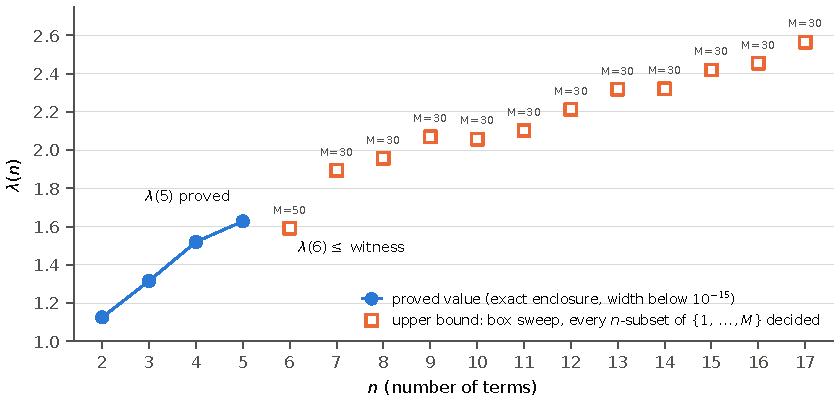
\includegraphics[width=\linewidth]{fig/lambda5-landscape.pdf}
\caption{The certified $\lambda$ landscape, $n=2,\dots,\LtMaxN$. Filled marks are proved values (Mercer at $n=2,3$; \cite{L4} at $n=4$; this paper at $n=5$). Hollow marks are the upper bounds of Table~\ref{tab:lambda}, each the best set in an exhaustive sweep of every $n$-subset of $\{1,\dots,M\}$; the sequence may lie below any of them. The value at $n=6$ is the witness bound of Theorem~\ref{thm:descent}.}\label{fig:landscape}
\end{figure}

\emph{Proof of Theorem~\ref{thm:descent}.} The certified minimum instrument gives
\[
\Ls\in\bigl[\,\LsixRatLo,\ \LsixRatHi\,\bigr],
\]
so $\lambda(6)\le-\Ls\le\LamSixUp$. Theorem~\ref{thm:main} gives $\lambda(5)\ge\LamFiveLo$. The comparison of the two rational endpoints, $\Lf^{\mathrm{hi}}<\Ls^{\mathrm{lo}}$, is decided exactly in the record (stage \texttt{targets}) and again in the battery; the ascent through $n=5$ is the analogous comparison with $L(1,2,3,4)$. \qed

\emph{Proof of Proposition~\ref{prop:seg}.} The record holds enclosures of $L(1,\dots,5)$ and $L(1,\dots,6)$ beside the two targets (Table~\ref{tab:seg}); each comparison is between exact rational endpoints. \qed

\begin{table}[t]\centering\small
\begin{tabular}{llll}\toprule
initial segment & $-L$ in & optimiser & $-L$ in\\\midrule
\SegRows
\bottomrule\end{tabular}
\caption{The initial segments against the sets of Theorems~\ref{thm:main} and \ref{thm:descent}; enclosures printed to six places, rounded outward.}\label{tab:seg}
\end{table}

Figure~\ref{fig:landscape} places the two theorems in the landscape. Nothing in the figure beyond $n=5$ is a value; the hollow marks are bounds from named boxes, and the shape they suggest, a slow rise with the $n=6$ dip, is a statement about those boxes.

\section{The independent walk}\label{sec:audit}

A second program, \texttt{tools/audit-lambda5.js}, shares no code with the symbolic engine. It computes inner products by direct trigonometric summation over the actual equispaced sets, decides condition membership by integer arithmetic on the record's condition vectors, reads from the record only data (vectors, deltas, the worklist, the target enclosure), and re-certifies from scratch every set its float screen cannot settle. On the box of all gcd-reduced $5$-sets with largest element at most \AudBox\ (\AudSets\ sets, \AudSeconds\ s, \AudDate) it decides five things, each able to fail only loudly.

\emph{The theorem.} Every set in the box dips strictly below $\Lf$ except $\{1,2,4,5,6\}$, which attains it: \AudRefuters\ refuters. \AudScreened\ sets were settled by the screen against the enclosure and the \AudExact\ set the screen could not settle was certified exactly; one screened set in every \AudSampleEvery\ (\AudScreenAudited\ in all) was then re-certified exactly, so the screen is itself audited rather than trusted.

\emph{The generic clause.} The two hypotheses of Lemma~\ref{lem:B} hold numerically: at the \AudGenericClosed\ sets (\AudGenericPct\%) on no positive condition the inner product is at most \AudWorstGeneric\ (against the symbolic $0$), and the weight's average is positive at every set in the box (least value \AudMinWeight).

\emph{Exhaustiveness.} The other \AudFamilyReached\ sets each satisfy at least one of the eight recorded family conditions; none is outside the reduction.

\emph{The symbolic layer.} The engine's model, inner product equals base plus the deltas of the active conditions, agrees with direct summation at every set in the box to \AudSymGap\ (worst at \AudSymWorstAt), and on the double-sum core to \AudCoreGap.

\emph{The obstruction, by mechanism.} On all \AudCorePoints\ core points in the box the complementary cosines cancel on $S(e,\pi)$ to a residual of \AudCancel, every classical atom at both anchors has strictly positive inner product (the least value over atoms, anchors and points is \AudClassicalWorst), and the comb's inner product is at most \AudCombWorst\ over the \AudCombPoints\ core points on no positive condition (the symbolic base is $\CoreBase$). The witness and \AudDilations\ dilations attain the target.

What the walk does not do, stated so that the status is exact: it does not enter the interior of the eight closure trees, the subfamily cones, the derived thresholds and the finite parts inside them. The $\lambda(4)$ audit does walk those for $\lambda(4)$ (\LfourAuditSets\ sets, \LfourAuditRecert\ finite-clause sets re-certified, box \LfourAuditBox, \LfourAuditDate), and the outside audit of \cite{Audit392} re-derived the $\lambda(4)$ families with its own code and swept every reduced $4$-set with largest element at most \LfourOutsideSweep; no equivalent exists yet for $\lambda(5)$. The battery \texttt{instruments/lambda56/battery.js} (\BatteryPass\ checks and \BatteryReds\ red controls, each a way the engine could lie, demonstrated to fail) re-derives the $\lambda(4)$ generic case before any $\lambda(5)$ claim is computed, walks the record so that a rotted record refuses rather than lingers, and pins the audit record against the target this document quotes.

\section{The Mercer program as a certified landscape}\label{sec:landscape}

The theorem sits inside a wider set of certificates produced by the same instruments, which we collect here with the scope of each stated. Two counting rules govern the tables: sets, boxes and candidate closed forms are different objects and are never summed into one figure, and nested sweeps are deflated, so a set re-decided in a wider box is counted once.

\subsection{Upper bounds on \texorpdfstring{$\lambda(n)$, $n=4,\dots,\LtMaxN$}{lambda(n), n = 4..\LtMaxN}}

\begin{table}[t]\centering\small
\resizebox{\linewidth}{!}{%
\begin{tabular}{rrlrrl}\toprule
$n$ & $M$ & witness $A_n$ & $\lambda(n)\le$ (rounds up) & sets decided & provenance\\\midrule
\LambdaRows
\bottomrule\end{tabular}}
\caption{Proposition~\ref{prop:lamtable}: the deepest box per $n$ in \texttt{certs/lambda-table.json}. Every row is an exhaustion with a conservation identity (integer kills at roots of unity, exact dyadic kills, full certification of survivors) that the numbers of this document re-add. ``The earlier table'' is a float-scouted table in the author's laboratory notes, reproduced here with every set decided exactly.}\label{tab:lambda}
\end{table}

\emph{Proof of Proposition~\ref{prop:lamtable}.} Each row of Table~\ref{tab:lambda} is an exhaustive sweep: a set is killed by an integer inequality at a root of unity of order $2,3,4$ or $6$ (where $2f_A$ is an integer), or by an exact evaluation at a dyadic point, or survives to full certification; the four counts add to $\binom Mn$ and the identity is re-added here. The bar is the certified value of the seed, stepped one unit in the last place down, so the witness cannot be killed by its own bar. \qed

The rows $n=4,\dots,12$ reproduce the earlier table, and $n=5$ and $6$ return exactly the sets of Theorems~\ref{thm:main} and \ref{thm:descent} as box optimisers (\LtFiveSets\ and \LtSixSets\ sets at $M=\LtFiveBox$ and $\LtSixBox$). The \LtRows\ recorded boxes contain \LtDeepened\ re-decisions of a settled $M=25$ answer at $M=30$; \LtConfirmed\ returned the incumbent and one improved the bound, at $n=\LtImprovedN$, where the wider box found \LtImprovedSet\ at $\LtImprovedBound$ against the shallow-box \LtImprovedPrev\ at $\LtImprovedPrevBound$. The confirmations are a decided negative over \LtConfirmedSets\ sets. Deflated, the table decides \LtDeepSets\ distinct sets; the \LtRedecided\ re-decided at a shallower $M$ are not counted again.

\subsection{Newman's \texorpdfstring{$0/1$}{0/1} minima: box maxima}

For $A$ a set of nonnegative integers, $|\sum_{a\in A}z^a|^2=|A|+2\sum_{i<j}\cos(a_j-a_i)\theta$ on the circle, an integer-coefficient cosine polynomial, so the same instrument decides $M(A)$; the differences form a multiset and the minimum is invariant under dilation and reversal. Table~\ref{tab:mu} gives the box maxima.

\begin{table}[t]\centering\small
\resizebox{\linewidth}{!}{%
\begin{tabular}{rrlrr}\toprule
$n$ & box $M$ & champion $A$ & $\mu(n)\ge$ (rounds down) & sets decided\\\midrule
\MuRows
\bottomrule\end{tabular}}
\caption{Proposition~\ref{prop:mu}: \texttt{certs/mu-table.json} (box 30, $n=\MuThirtyLo,\dots,\MuThirtyHi$) and \texttt{certs/mu-table-40.json} (box 40, $n=\MuFortyLo,\dots,\MuFortyHi$). Sets are $\{0\}\cup B$ with $B$ an $(n-1)$-subset of $\{1,\dots,M\}$. A box maximum is a lower bound on $\mu(n)$ and a completeness statement about its box, not a value.}\label{tab:mu}
\end{table}

\begin{sloppypar}
The $n=9$ row validates the instrument against the printed record: the witness of Boyd \cite{Bo86}, which is \BoydNine, comes back as one of the \NineSurvivors\ survivors of the sweep, with $M\ge\BoydNineFloor$, and the box maximum stands above it. The wider box lifted every floor it touched (\MuLiftList), which is the reason the dips in the box-30 column at larger $n$ are read as box crowding and not as mathematics. Deflated, the two tables decide \MuDistinctSets\ distinct sets (\MuNested\ lie in both boxes). No priority is claimed for any row: Boyd's survey has not been read first-hand in this laboratory, so each row is a first certificate over a named box, re-checkable by the repository's batteries, and nothing more.
\end{sloppypar}

\subsection{The \texorpdfstring{$\mu(5)$}{mu(5)} ladder, and an equality}

\begin{table}[t]\centering\small
\begin{tabular}{rrrrr}\toprule
$m$ & $\mu(5)\le1+\pi/m$ (rounds up) & fraction rows examined & tuples closed & time\\\midrule
\LadderRows
\bottomrule\end{tabular}
\caption{Theorem~\ref{thm:ladder}: \texttt{certs/mercer-mu5.json}, one rung per $m$. The rows $m=5$ and $6$ reproduce Mercer's Tables~5 and 6--7 exactly; the rungs $m\ge7$ are new. The pinned source is \texttt{corpus/sources/mercer2019\_integers.pdf} (sha256 \LadderPdfSha\dots).}\label{tab:ladder}
\end{table}

\emph{Proof of Theorem~\ref{thm:ladder}.} For $(0,a,b,c,d)$ with the differences not all bounded by the gcd argument, Mercer's Lemma~6.2 gives $|1+z^a+z^b+z^c+z^d|\le1+\pi g_i/d$ (or $/c$) at some $|z|=1$ for each of six inner gcds $g_i$. If some ratio is at most $1/m$ the bound holds outright; otherwise the six ratios $r,s,t,u,v,w$ are reduced fractions in $(0,1)$ with denominators below $m$ satisfying $r+s=t$, $u+v=w$, $r<u$, $s<v$ and $r(1+v)=u(1+s)$, and each admissible quadruple pins the tuple up to scale. That reduction is Mercer's and is consumed. For each $m$ the search over all reduced fractions with denominator below $m$ is run in exact rational arithmetic (Table~\ref{tab:ladder}, third column), and each derived tuple is closed by one exact evaluation of $|f|^2$ at a candidate point against the exact bar $(1+\pi_{\mathrm{lo}}/m)^2$, with $\pi_{\mathrm{lo}}$ a dyadic rational below $\pi$ from a certified enclosure (an attained value is an upper bound on a minimum). At $m=\LadderTop$ this is \LadderTopExamined\ candidate rows and \LadderTopTuples\ tuples; in all, \LadderTuples\ tuples across \LadderRungs\ rungs, none failed and none refused. With Proposition~\ref{prop:eq}, $1\le\mu(5)\le1+\pi/\LadderTop$. \qed

\emph{Proof of Proposition~\ref{prop:eq}.} With $y=\cos\theta$ and $G(y)=|f|^2$ for $A=\{0,1,2,6,9\}$, $G(-1)=1$, and $G(y)-1=(y+1)^{\EqK}H(y)$ exactly, with $\deg H=\EqDegH$, $H(-1)=\EqHm>0$ and $H(1)=\EqHp>0$; a Sturm chain of the square-free part of $H$ counts zero roots of $H$ in $(-1,1]$, so $|f|^2\ge1$ on the circle with equality exactly at $y=-1$. This is a tie that no enclosure can decide; it is decided in integer arithmetic end to end, and re-proved at every build of the report page. Mercer observed the value and suspected $\mu(5)=1$. \qed

\subsection{Merits at fixed \texorpdfstring{$n$}{n}}

Chowla's normalisation is the merit $c(A)=-L(A)/\sqrt{|A|}$, and his conjecture is that $c$ is bounded below. The generation front of the repository, pointed at the problem on \ChowlaDate, certified the best merit its set-walk proposer found at each of five sizes against the best classical set at the same size (Table~\ref{tab:chowla}). Each row is a fact about one $n$: an upper bound on the infimum of $c$ over sets of that size, decided exactly for the set beside it. The merits rise from \ChowlaFirstC\ at $n=\ChowlaFirstN$ to \ChowlaLastC\ at $n=\ChowlaLastN$, which is consistent with Chowla's conjecture and proves nothing about it.

\begin{table}[t]\centering\small
\begin{tabular}{rrrlr}\toprule
$n$ & $\max A\le$ & $c(A)\le$ & classical set & its $c\le$\\\midrule
\ChowlaRows
\bottomrule\end{tabular}
\caption{\texttt{certs/chowla-records.json}: certified merits of the best set found at each size and of the best classical set at that size, both rounded up.}\label{tab:chowla}
\end{table}

\section{\texorpdfstring{$\lambda(6)$}{lambda(6)}: the open front}\label{sec:six}

The same generic move at $n=6$, on $S(f,\pi)$ with $w=2(1-\cos e\theta)^2$ and $g_0=\frac23$, has base $0$ and dip $\GenDip$, which clears $\Ls$, and raises \SixConditions\ conditions, \SixPositive\ positive and \SixNegative\ self-closing; the witness $\{1,2,4,6,7,8\}$ activates three with delta sum $\SixEscapeSum$ and escapes, as it must. Table~\ref{tab:six} gives the state of the ten families. Nine are closed in the record, by \SixDots\ dot theorems, \SixClosures\ closures, \SixSets\ finite sets and \SixOnto\ coverage points, with the only skipped set the witness; the heaviest, \SixHeaviest, took \SixHeaviestTime\ and \SixHeaviestSets\ finite sets. The tenth, \SixOpen, is not closed.

\begin{table}[t]\centering\small
\begin{tabular}{llcrrrrr}\toprule
family & delta & status & dot thms & closures & finite sets & coverage pts & time\\\midrule
\SixRows
\bottomrule\end{tabular}
\caption{The ten exception families of the $\lambda(6)$ generic case; counts as the run recorded them (a memoised subtree is counted once). The open family has no stage in the record.}\label{tab:six}
\end{table}

What is known about the open family is in the session log and not in any certificate, so we report it as such. The log records three runs of the closer on \SixOpen\ dying at the same node: one was still computing after about \LogOpenHours\ hours, a later one after \LogOpenHoursMax\ hours at node \LogOpenNode\ of its tree, and none produced a verdict. A traced twin of the run, started in an isolated copy so that it could not touch the record, reproduced the stall: \LogTwinNodes\ nodes in its first \LogTwinSeconds\ seconds, then one node, number \LogStallNode\ at depth \LogStallDepth\ with \LogStallDof\ free parameters, holding the process for more than \LogStallMinutes\ minutes at the time of the entry and never released; a closed family traced the same way as a baseline ran \LogBaseNodes\ nodes in \LogBaseMinutes\ minutes at a steady \LogBaseRate\ nodes per minute with maximum depth \LogBaseDepth. The log's diagnosis is therefore not a larger tree but a single two-parameter endgame node whose cost explodes inside the closer's capped adaptive coverage boxes, and its conclusion is that the fix is mathematical, a better mechanical shape for that cone or a different box schedule, and not more hours. Until it lands, $\lambda(6)$ has the upper bound of Theorem~\ref{thm:descent} and no value here; $\lambda(6)=-\Ls$ remains Mercer's conjecture.

\section{What is not claimed}\label{sec:notclaimed}

Theorem~\ref{thm:main} is machine-derived from a public record and has been audited independently at the level of the theorem, the first level of the reduction and the obstruction; the interior of its eight closure trees has not been walked by any second program, and no human referee has read it. The value $\lambda(6)$ is not claimed, and neither is the uniqueness of its optimiser; Theorem~\ref{thm:descent} is a comparison of a proved value with an exhibited set. Whether $\lambda(5)$ is expressible in radicals is not decided. The rows of Table~\ref{tab:lambda} are upper bounds on an infimum over named boxes; the rows of Table~\ref{tab:mu} are lower bounds over named boxes; neither table orders its values across $n$, and neither claims a first in the printed record. Theorem~\ref{thm:ladder} consumes Mercer's reduction as a proved external statement and certifies only the two computer-aided components he described. The merits of Table~\ref{tab:chowla} say nothing about the asymptotic problem. The novelty claimed is the decision grammar and the record: the arithmetic (exact rationals, Sturm sequences, outward rounding) is standard, and the statement and strategy are Mercer's.

\cmrepro{\begin{sloppypar}
The campaign record is \texttt{certs/lambda56-campaign.json} (\CampaignDate, git \CampaignGit; \CampaignHours\ h of wall time for the recorded stages, written incrementally after every stage). It is rebuilt by \texttt{node tools/run-lambda56-campaign.js}, which takes hours; the variable \texttt{ONLY} names one family to run. The independent walk is \texttt{node tools/audit-lambda5.js}, with the box as its optional argument; it writes \texttt{certs/lambda5-audit.json} (\AudDate, git \AudGit; \AudSeconds\ s at box \AudBox). The battery is \texttt{node instruments/lambda56/battery.js}, about five seconds. The report page is built by \texttt{node tools/build-report-lambda5.js}; at every build it re-derives the target enclosure, the minimal polynomial after its two calibrations, the generic case, the double-sum-core theorem with its eight refusals, the record walk and a sample of finite certificates.

The companion records, each with the tool that writes it:
\begin{itemize}\setlength{\itemsep}{0pt}
\item \texttt{certs/lambda4-campaign.json} and \texttt{certs/lambda4-audit.json} (\LfourCampaignDate), the $\lambda(4)$ companion;
\item \texttt{certs/lambda-table.json}, by \texttt{tools/run-lambda-table.js};
\item \texttt{certs/mu-table.json} and \texttt{certs/mu-table-40.json}, by \texttt{tools/run-mu-table.js};
\item \texttt{certs/mercer-mu5.json}, by \texttt{tools/run-mercer-mu5.js} with the argument 20;
\item \texttt{certs/chowla-records.json}, by \texttt{tools/run-chowla-front.js}.
\end{itemize}
The Mercer-program page, \texttt{tools/build-report-mercer.js}, re-certifies every champion and re-proves the equality at every build. The instruments are \texttt{instruments/lambda4/} (forms, dot, estimates, engine), \texttt{instruments/lambda56/close.js} (the tree driver) and \texttt{instruments/trigmin/} (certify-min, lambda, newman, sweep, mercer6, minpoly).

The macros of this document are written by \texttt{node tools/paper-numbers/lambda5.js}, which also runs the battery and the sub-second live derivations; the figure by \texttt{tools/paper-numbers/lambda5-figs.py}; the document is compiled by \texttt{node tools/build-paper-tex.js lambda5}, here at git \RepoCommit. The one pinned source is Mercer's paper, \texttt{corpus/sources/mercer2019\_integers.pdf}.
\end{sloppypar}}

\begin{thebibliography}{99}
\bibitem{Me19} I.~Mercer, Finite searches, Chowla's cosine problem, and large Newman polynomials, Integers 19 (2019), \#A4; arXiv:1709.06612.
\bibitem{Ch65} S.~Chowla, Some applications of a method of A.~Selberg, J.~Reine Angew.\ Math.\ 217 (1965), 128--132.
\bibitem{UU60} M.~Uchiyama and S.~Uchiyama, On the cosine problem, Proc.\ Japan Acad.\ 36 (1960), 475--479.
\bibitem{Co60} P.~J.~Cohen, On a conjecture of Littlewood and idempotent measures, Amer.\ J.\ Math.\ 82 (1960), 191--212.
\bibitem{Ru04} I.~Z.~Ruzsa, Negative values of cosine sums, Acta Arith.\ 111 (2004), 179--186.
\bibitem{Be25} B.~Bedert, Polynomial bounds for the Chowla cosine problem, arXiv:2509.05260 (2025), as cited in \cite{L4}.
\bibitem{JMTZ25} Jin, Milojevi\'c, Tomon and Zhang, arXiv:2509.03490 (2025), the asymptotic side, as cited in \cite{L4}.
\bibitem{CFF83} D.~M.~Campbell, H.~R.~P.~Ferguson and R.~W.~Forcade, Newman polynomials on $|z|=1$, Indiana Univ.\ Math.\ J.\ 32 (1983), 517--525.
\bibitem{Go92} B.~Goddard, Finite exponential series and Newman polynomials, Proc.\ Amer.\ Math.\ Soc.\ 116 (1992), 313--320.
\bibitem{Bo86} D.~W.~Boyd, Large Newman polynomials, in Diophantine Analysis (Kensington, 1985), 159--170, London Math.\ Soc.\ Lecture Note Ser.\ 109, Cambridge Univ.\ Press, 1986.
\bibitem{L4} C.~Toledo, The value of $\lambda(4)$: a machine-derived proof that $\lambda(4)=-L(1,2,3,4)$, completing the program of Mercer's Section~5, cert-machine draft v0.9 (2026), doi:10.5281/zenodo.22225861; report page \url{https://carlostoledo.co/reports/lambda4.html}.
\bibitem{Audit392} rainrzk, erdos510-lambda4-audit, an independent re-certification of \cite{L4}, posted on teorth/erdosproblems, issue~392, 30~September 2026. Repository: \url{https://github.com/rainrzk/erdos510-lambda4-audit}.
\bibitem{EP510} Erd\H{o}s problem \#510, \url{https://www.erdosproblems.com/510}.
\bibitem{L5page} C.~Toledo, $\lambda(5)$: the report page and the campaign record, \texttt{certs/lambda56-campaign.json} and \texttt{certs/lambda5-audit.json} in the cert-machine repository (2026). Page: \url{https://carlostoledo.co/reports/lambda5.html}.
\bibitem{Mpage} C.~Toledo, The Mercer program: $\mu$, $\lambda$, and a forty-year bracket, \url{https://carlostoledo.co/reports/mercer-program.html} (2026).
\end{thebibliography}

\end{document}
